\documentclass[12pt,a4paper]{article}
\usepackage[UTF8]{ctex}
\usepackage{amsmath,amssymb}
\usepackage{xcolor}
\usepackage{hyperref}
\usepackage{geometry}
\usepackage{graphicx}
\geometry{margin=2.5cm}

\title{Quantum Interface / 量子接口}
\author{QuoNic}
\date{}

\begin{document}
\maketitle

\begin{center}
\textbf{Language / 语言特性} | 难度：初级 | 预计时间：5 分钟
\end{center}

\tableofcontents
\newpage

\section{为什么需要？}

量子接口是 QuoNic 框架的核心 API。

\subsection{经典局限}
\begin{itemize}
  \item 经典编程接口无法直接操作量子态
  \item 需要量子抽象层
\end{itemize}

\subsection{量子优势}
\begin{itemize}
  \item 量子接口提供了统一的量子编程 API
  \item 支持多种量子后端
  \item 简化量子编程
\end{itemize}

\subsection{实际应用}
\begin{itemize}
  \item 量子编程
  \item 量子算法开发
  \item 量子硬件访问
\end{itemize}

\section{快速上手}

\begin{verbatim}
from quonic import qgate, qshow
from quonic.gates import H

# 量子接口
qgate(H, 0)
qshow()
\end{verbatim}

\textbf{预期输出}：
\begin{verbatim}
backend: native | shots: 1024
Result:
  |0>     512  ( 50.0%)
  |1>     512  ( 50.0%)
\end{verbatim}

\section{原理详解}

\subsection{电路图}

\begin{center}
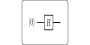
\includegraphics[width=0.6\textwidth]{../../images/qi_circuit.svg}
\end{center}

\subsection{数学推导}

量子接口提供统一的量子编程 API：
\begin{itemize}
  \item \texttt{qgate(gate, qubit)}: 施加量子门
  \item \texttt{qshow()}: 测量并显示结果
  \item \texttt{reset()}: 重置量子态
\end{itemize}

\subsection{几何解释}

量子接口在 Bloch 球上操作量子态。qgate() 施加量子门，qshow() 测量并显示结果。

\section{代码详解}

\begin{verbatim}
from quonic import qgate, qshow, reset
from quonic.gates import H, CX

# qgate(gate, qubit): 施加量子门
qgate(H, 0)      # Hadamard 门
qgate(CX, 0, 1)  # CNOT 门

# qshow(): 测量并显示结果
qshow()

# reset(): 重置量子态
reset()
\end{verbatim}

\section{进阶用法}

\subsection{场景 1：选择后端}

\begin{verbatim}
from quonic import qgate, qshow
from quonic.gates import H

# 选择后端
qshow(backend='native')
qshow(backend='qiskit')
qshow(backend='cirq')
\end{verbatim}

\subsection{场景 2：设置 shots}

\begin{verbatim}
from quonic import qgate, qshow
from quonic.gates import H

# 设置测量次数
qgate(H, 0)
qshow(shots=4096)
\end{verbatim}

\section{适用场景}

\subsection{量子编程}

量子接口提供统一的量子编程 API。开发者可以使用相同的代码在不同量子硬件上运行。

\subsection{量子算法开发}

量子接口简化量子算法开发。开发者可以专注于算法逻辑，不需要关心底层实现。

\section{常见问题}

\subsection{量子接口支持哪些后端？}

QuoNic 支持多种后端，包括 native、qiskit、cirq、cudaq 等。

\subsection{量子接口的性能如何？}

量子接口的性能取决于后端。native 后端最快，其他后端可能有额外开销。

\section{学习路径}

\subsection{前置知识}
\begin{itemize}
  \item 量子比特
  \item 量子门
  \item 量子测量
\end{itemize}

\subsection{继续学习}
\begin{itemize}
  \item 量子算法
  \item 量子电路
  \item 量子硬件
\end{itemize}

\section{完整示例代码}

\subsection{示例 1：基本量子接口}

\begin{verbatim}
from quonic import qgate, qshow
from quonic.gates import H

qgate(H, 0)
qshow()
\end{verbatim}

\section{下载}

\begin{itemize}
  \item [qi.py](https://github.com/ChrisLee0721/QuoNic/blob/main/examples/qi/qi.py)
\end{itemize}

\end{document}
